In mean-field variational inference, the E-step in \eqref{eq:e_step} is often optimized by coordinate descent in the parameters of the variational distribution. 
The coordinate descent updates can be derived in closed form in the special case of exponential family models that are conditionally conjugate~\cite{Blei_2017_vi_review}. 

In our setting of amortized variational inference, stochastic 
optimization procedures have been employed with modern 
auto-differentiation tools to avoid the need for deriving 
analytic updates. Examples include black-box variational inference (BBVI)~\cite{ranganath2013black} 
and automatic-differentiation variational inference (ADVI)~\cite{kucukelbir2016automatic}. The latter 
is closely related to the reparameterization trick that \cite{kingma2013autoencoding, rezende2014stochastic} proposed to train deep generative models using the KL objective. 
These approaches all sample latent variables from $q_\eta$ and produce an unbiased estimate 
for the gradient of the KL; the optimization is done with stochastic gradient descent. 

However, the reparameterization trick does not apply when a latent variable is discrete, in our case, the number of stars $N$. Alternatively, the REINFORCE estimator~\cite{Williams1992reinforce}, which BBVI adapts, produces an unbiased stochastic gradient for both continuous and discrete latent variables. However, it often suffers from high variance in practice and the resulting stochastic optimization is slow. 

Stochastic gradients are difficult to compute in the E-step because the integrating distribution depends on the optimization parameter, $\eta$. 
The wake-sleep algorithm, originally proposed by~\cite{Hinton1995wake_sleep}, replaces the 
E-step objective with 
\begin{align}
    \argmin_{\eta} \Expect_{\tilde x \sim p(\tilde x)}\Big[\KL(p_\phi(\theta | \tilde x) \| q_\eta(\theta | \tilde x)\Big]
    \label{eq:sleep_obj}
\end{align}
called the {\itshape sleep phase}. We will see in Section~\ref{sec:sleep_details} that a simple gradient estimator can be derived for the sleep phase objective, without 
reparameterization or REINFORCE. 

We comment on two key differences between the sleep objective and the E-step (equation~\eqref{eq:e_step}). First note the difference in ordering of arguments to the $\KL$. 
While optimizing $\KL(q\|p)$ in equation~\eqref{eq:e_step} does not depend on the intractable 
data likelihood $p_\phi(x)$, the $\KL$ with arguments reversed does. 
As will be detailed in Section~\ref{sec:sleep_details}, the outer expectation over the data makes this optimization objective tractable without dependence on $\log P(x)$. 

The expectation over the data also gives different meaning to the sleep objective. The E-step objective seeks $\eta$ to minimize the $\KL$ between $P_\phi(\theta | x)$ and $q_\eta(\theta | x)$ {\itshape for fixed, observed data $x$},
in this case the $H\times W$ image. In contrast, the sleep objective seeks to minimize the $\KL$ {\itshape averaged over all possible data. } In other words, the target is no longer an approximate posterior for observed data, but rather an approximate posterior that is ``good on average" over possible data .

Moreover, ``possible data" is defined under our generative model from Section~\ref{sec:gen_model}. In order for $q_\eta(\theta | x)$ to be a good approximation to
the true posterior when $x$ is observed data, then it is imperative that our generative model $p_\phi(x)$ well-approximates the true underlying data-generating mechanism. 

Therefore, a {\itshape wake phase} is employed to tune the model parameters. The wake-phase objective is
\begin{align}
    \phi_{t} = \argmax_{\phi} \; \Expect_{q_{\eta}(\theta | x)}\Big[\log p_\phi(x, \theta)\Big], 
    \label{eq:wake_elbo}
\end{align}
which is equivalent to the M-step in variational EM (equation~\ref{eq:m_step}). 

Stochastic gradients are easy to compute in the wake phase (M-step). Because the integrating distribution does not depend on the optimization parameter $\phi$ in the wake phase, unbiased stochastic gradients are computed simply as 
\begin{align}
    \nabla_\phi \log p_\phi(x, \theta) \quad \text{ for } \theta\sim q_\eta
    \label{eq:mstep_grad}
\end{align}
While the E-step is not conducive to simple gradient estimators, we will see in Section~\ref{sec:sleep_details} that our sleep-phase objective
results in a similarly straightforward gradient estimator as in equation~\eqref{eq:mstep_grad}. However,
we note that a consequence of replacing the E-step with the sleep phase is that the wake-sleep algorithm no longer targets a singular objective like that of equation~\eqref{eq:em_obj}. 

% Equation~\eqref{eq:wake_elbo} is equivalent to maximizing the ELBO in equation~\eqref{eq:elbo} with respect to model parameters $\phi$. 
% Since maximizing the ELBO is equivalent to 
% minimizing the $\KL$, we can also express the wake-phase objective as 
% \begin{align}
%     \phi_{t} = \argmin_{\phi} \; \mathrm{KL}\Big[\,q_\eta(\theta | x)\, \| \,p_\phi(\theta | x )\,\Big]. 
% \end{align}

% In summary, given an initial $\eta_0$, $\phi_0$, and data $x$,
% for $t = 1, ..., T$, the wake-sleep algorithm alternates between two objectives: 
% \begin{align}
%     \text{{\bf Sleep: }} & 
%     \eta_{t} = \argmin_\eta \; \Expect_{p_{\phi_{t - 1}}(\tilde x)}\Big[\KL\big ( p_{\phi_{t - 1}}(\theta | \tilde x)\| q_{\eta}(\theta |\tilde x)\big)\Big]
%     \label{eq:sleep_kl}\\
%     \text{{\bf Wake: }} & \phi_{t} =  \argmin_{\phi} \; \mathrm{KL}\Big[\,q_{\eta_t}(\theta | x)\, \| \,p_\phi(\theta | x )\,\Big]. 
%     \label{eq:wake_kl}
% \end{align}
% order to construct an approximate posterior. In the wake phase, we reveal the observed data $x$ and optimize model parameters $\phi$ so that our data-generating process aligns as closely as possible with the true data. 

\subsubsection{Decomposing the sleep objective}
\label{sec:sleep_details}
In this section, we decompose the sleep-phase objective in equation~\eqref{eq:sleep_obj} to examine its properties. 
We take $\phi$ as fixed in this section, and drop the explicit dependence of $p$ on $\phi$.

First, we show that the objective does not depend on the intractable term $p(x)$. 
We write
\begin{align}
 \argmin_{\eta} \; & \mathbb{E}_{\tilde x \sim p(\tilde x)}\Big[ \mathrm{KL}(P(\theta | \tilde x) \| q_\eta(\theta | \tilde x)\Big] \\
  &=\argmin_{\eta} \; \mathbb E_{p(\tilde x)}\Big[\mathbb E_{p(\theta | \tilde x)}\Big(\log p(\theta | \tilde x) - \log q_\eta(\theta | \tilde x) \Big)\Big]\\
&=\argmin_{\eta} \; \mathbb E_{p(\tilde x)}\Big[\mathbb E_{P(\theta | \tilde x)}\Big( - \log q_\eta(\theta | \tilde x) \Big)\Big]\\
&=\argmin_{\eta} \; \mathbb E_{p(\tilde x, \theta)}\Big[- \log q_\eta(\theta | \tilde x) \Big]\label{eq:sleep_loss_simple}
\end{align}
Crucially, the integrating distribution is $P$, which does not depend on the optimization parameter $\eta$.
In the E-step of variational EM (equation~\eqref{eq:e_step}), the integrating distribution is $q_\eta$, resulting in the need for reparameterization or other adjustments to compute stochastic gradients. 
Here, unbiased stochastic gradients can be obtained simply as 
\begin{align}
    g = -\nabla_\eta \log q_\eta(\theta | \tilde x) \quad \text{ for } (\theta, \tilde x)\sim p
\end{align}

In other words, we simulate {\itshape complete} data $(\theta, \tilde x)$ from our generative model and evaluate the loss $-\log q_\eta(\theta | \tilde x)$. 
This loss encourages $q_{\eta}(\theta | \tilde x)$ to map images $\tilde x$ to a probability distribution with large mass on $\theta$.

We examine the loss $-\log q_\eta(\theta | \tilde x)$ more closely. Recall that $q_\eta$ factorizes over image tiles. Having sampled the full image catalog $\theta$ 

TODO: I messed up the notation now ... 

and the $H\times W$ image $\tilde x$ from $P$, we convert the latent variables to their patch parameterization $(N^k, \ell^k, f^k)_{k = 1}^K$. 

For a given image patch, the latent variables $N^k$, $\ell^k$, $f^k$ also factorize in $q$, so 
\begin{align}
    - \log q_\eta(N^k, \ell^k, f^k | \tilde x) = 
        - \log q_\eta(N^k | \tilde x) 
        - \log q_\eta(\ell^k | \tilde x) 
        - \log q_\eta(f^k | \tilde x). 
        \label{eq:sleep_loss_decomp}
\end{align}
We examine each term separately. On patch $k$, the number of stars $N^k$ is categorical with parameter $\omega^k$. The loss function for the number of stars becomes
\begin{align}
    - \log q_\eta(N^k | \tilde x) = -\sum_{n = 0}^{N_{max}} 1\{N^k = n\} \log \omega^k_n, 
\end{align}
the usual cross-entropy loss for a multi-class classification problem. 

For the last two terms, recall that location coordinates are logit-normal and fluxes are log-normal. For a given index $(i, N)$ let $y^k_{i,N}$ generically denote either the 
logit-location or log-flux for that star, 
and let $\mu^k_{i,N}$ and $\sigma^{k}_{i,N}$ generically denote its variational parameters,
the mean and standard deviation of a Gaussian. Then the losses in the last two terms of equation~\ref{eq:sleep_loss_decomp} are of the form 
\begin{align}
    -\log q_\eta(y^k_{i,N} | \tilde x) = 
        \frac{1}{2(\sigma^{k}_{i,N})^2}(y^k_{i,N} - \mu^k_{i,N})^2
         + \log\sigma^{k}_{i,N}
         + \frac{1}{2}\log(2\pi)
\end{align}
We also give an interpretation: $y_{i,N}$ is the true, simulated latent variable (either logit-location or log-flux); $\mu^k_{i,N}$ is the predicted value for that latent variable of the neural network. $\sigma^{k}_{i,N}$ is also outputted by the neural network, representing uncertainty -- the second term encourages small uncertainties, but this is 
balanced by the scaling of the error $(y^k_{i,N} - \mu^k_{i,N})^2$ in the first term. 

In summary, the sleep-phase results in a supervised learning problem on complete data simulated from our generative model. 

\subsubsection{Reverse versus forward KL}
\label{sec:kl_q_p}
TODO: something about forward KL overestimates uncertainties, see Figure~\ref{fig:kl_q_p_schematic}. 

\begin{figure}[!h]
    \centering
    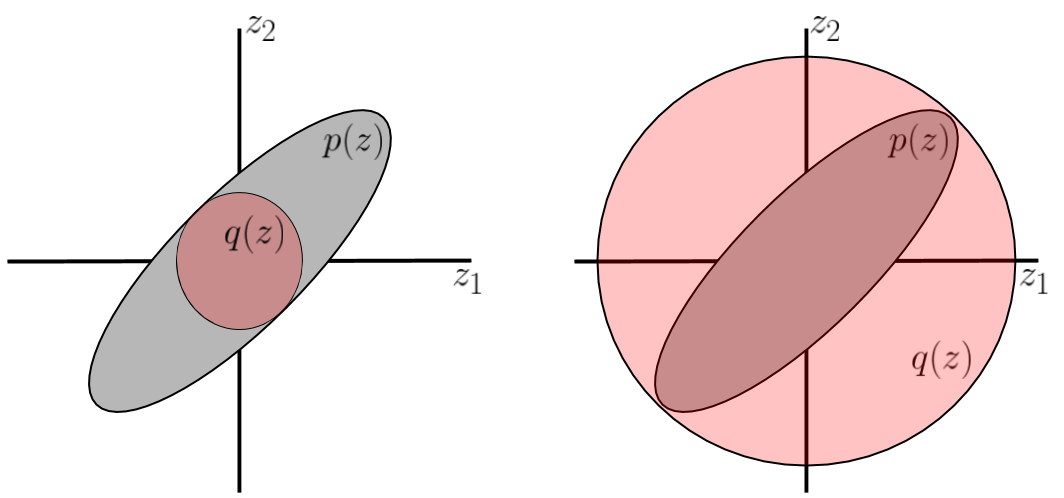
\includegraphics[width = 0.5\textwidth]{figures/kl_q_p_schematic.png}
    \caption{A toy example where the true distribution is a bivariate Gaussian on 
    $\theta = (\theta_1, \theta_2)$ with positively correlated components. 
    $q$ is a mean-field variational approximation. Left, the optimal $q$ found 
    optimizing $\KL(q\|p)$; right, the optimal $q$ found optimizing $\KL(p\|q)$. }
    \label{fig:kl_q_p_schematic}
\end{figure}

% \begin{itemize}
%     \item Number of stars $N$ is {\color{red}{\bf categorical}} with parameter $\omega$. 
%     \item Locations $\ell_n$ are {\color{blue}{\bf logitnormal}} with parameters $\mu_{\ell, n}$ and $\nu_{\ell, n}$
%     \item Fluxes $f_n$ are {\color{orange}{\bf lognormal}} with parameters $\mu_{f, n}$ and $\sigma^2_{f, n}$. 
% \end{itemize}
